%%%%%%%%%%%%%%%%%%%%%%% file template.tex %%%%%%%%%%%%%%%%%%%%%%%%%
%
% This is a general template file for the LaTeX package SVJour3
% for Springer journals.          Springer Heidelberg 2010/09/16
%
% Copy it to a new file with a new name and use it as the basis
% for your article. Delete % signs as needed.
%
% This template includes a few options for different layouts and
% content for various journals. Please consult a previous issue of
% your journal as needed.
%
%%%%%%%%%%%%%%%%%%%%%%%%%%%%%%%%%%%%%%%%%%%%%%%%%%%%%%%%%%%%%%%%%%%
%
% First comes an example EPS file -- just ignore it and
% proceed on the \documentclass line
% your LaTeX will extract the file if required
%
\RequirePackage{fix-cm}
%
%\documentclass{svjour3}                     % onecolumn (standard format)
%\documentclass[smallcondensed]{svjour3}     % onecolumn (ditto)
%\documentclass[smallextended]{svjour3}       % onecolumn (second format)
\documentclass[twocolumn]{svjour3}          % twocolumn
%
\smartqed  % flush right qed marks, e.g. at end of proof
%
% The following packages can be found on http:\\www.ctan.org
\usepackage{graphics} % for pdf, bitmapped graphics files
%\usepackage{epsfig} % for postscript graphics files
%\usepackage{mathptmx} % assumes new font selection scheme installed
%\usepackage{times} % assumes new font selection scheme installed
\usepackage{amsmath} % assumes amsmath package installed
\usepackage{amssymb}  % assumes amsmath package installed
\usepackage{url}
    % By default the URLs are put in typewriter type in the body and the
    % bibliography of the document when using the \url command.  If you are
    % using many long URLs you may want to uncommennt the next line so they
    % are typeset a little smaller.
\renewcommand{\UrlFont}{\small\tt}
\usepackage{graphicx}
\usepackage{listings}
\usepackage{color}
\usepackage[tight]{subfigure}
\usepackage{algorithm}
\usepackage{algorithmic}

\usepackage{listings}
  \usepackage{courier}
 \lstset{
         %basicstyle=\footnotesize\ttfamily, % Standardschrift
         basicstyle=\scriptsize\ttfamily, % Standardschrift
         %numbers=left,               % Ort der Zeilennummern
         numberstyle=\tiny,          % Stil der Zeilennummern
         %stepnumber=2,               % Abstand zwischen den Zeilennummern
         numbersep=5pt,              % Abstand der Nummern zum Text
         tabsize=1,                  % Groesse von Tabs
         extendedchars=true,         %
         breaklines=true,            % Zeilen werden Umgebrochen
         keywordstyle=\color{red},
            frame=b,
 %        keywordstyle=[1]\textbf,    % Stil der Keywords
 %        keywordstyle=[2]\textbf,    %
 %        keywordstyle=[3]\textbf,    %
 %        keywordstyle=[4]\textbf,   \sqrt{\sqrt{}} %
         stringstyle=\color{white}\ttfamily, % Farbe der String
         showspaces=false,           % Leerzeichen anzeigen ?
         showtabs=false,             % Tabs anzeigen ?
         xleftmargin=17pt,
         framexleftmargin=17pt,
         framexrightmargin=5pt,
         framexbottommargin=4pt,
         %backgroundcolor=\color{lightgray},
         showstringspaces=false      % Leerzeichen in Strings anzeigen ?
 }
 \lstloadlanguages{% Check Dokumentation for further languages ...
         %[Visual]Basic
         %Pascal
         %C
         %C++
         XML
         %HTML
         %Java
 }
    %\DeclareCaptionFont{blue}{\color{blue}}

  %\captionsetup[lstlisting]{singlelinecheck=false, labelfont={blue}, textfont={blue}}
  \usepackage{caption}
    %\DeclareCaptionFont{white}{\color{white}}
    %\DeclareCaptionFormat{listing}{\colorbox[cmyk]{0.43, 0.35,0.35,0.01}{\parbox{\textwidth}{\hspace{15pt}#1#2#3}}}
    \DeclareCaptionFormat{listing}{\colorbox[cmyk]{0, 0,0,0}{\parbox{\columnwidth}{\hspace{15pt}#1#2#3}}}
    %\captionsetup[lstlisting]{format=listing,labelfont=white,textfont=white,singlelinecheck=false, margin=0pt, font={bf,footnotesize}}
    \captionsetup[lstlisting]{format=listing,singlelinecheck=false, margin=0pt}

\graphicspath{{./}{./figures/}}

%-----------------------------------------------------------------------------
% DOCUMENT
%-----------------------------------------------------------------------------
\begin{document}

%Architecture for the generation of multi-UAS plans using symbolic and task allocation planners

\title{Architecture for the automatic generation of plans for multiple UAS from a generic mission description  
\thanks{This work has been partially supported by the ARCAS Project (FP7-ICT-287617) funded by the EU FP7 and the RANCOM Project (P11-TIC-7066).}}
%\subtitle{Do you have a subtitle?\\ If so, write it here}

\titlerunning{Architecture for the generation of plans for multiple UAS}        % if too long for running head

\author{Jorge Mu\~{n}oz-Morera        \and
        Ivan Maza \and
        Fernando Caballero \and
        Anibal Ollero
}

%\authorrunning{Short form of author list} % if too long for running head

\institute{J. Mu\~{n}oz-Morera, I. Maza, F. Caballero and A. Ollero are with Grupo de Robotica, Visi\'on y Control,
        Universidad de Sevilla, Spain. E-mails: {\tt\small jorgemunoz@us.es, imaza@us.es, fcaballero@us.es, aollero@us.es}
}

\date{Received: date / Accepted: date}
% The correct dates will be entered by the editor

\maketitle

%-----------------------------------------------------------------------------
% ABSTRACT
%-----------------------------------------------------------------------------
\begin{abstract}
A planning approach for a platform composed of multiple unmanned aerial systems is presented in this paper. The research activities are focused on the interoperability, task allocation 
and task planning problems within the system. In order to tackle with the interoperability problem between the vehicles of the platform and other external systems, C-BML has been chosen as the standard language to formalize the description of the missions. Regarding the planning problems involved, several planners have been applied to solve them: a task allocation planner to create an initial assignment of tasks to vehicles, a symbolic planner for high-level reasoning and tools for geometric reasoning. The main contribution of the paper is the capability of the system to automatically generate low level plans for each of the vehicles from a mission described in C-BML. The approach has been tested in missions involving multiple surveillance and 3D map generation tasks and the paper includes experimental results.   

\begin{keywords}
\\
Symbolic Planning; \and Task Planning; \and Task Allocation; \and Multiple UAS; \and Interoperability
\end{keywords}

\end{abstract}

\section{Introduction and Related Work}
\label{sec:intro}

Although Unmanned Aerial Systems (UAS) have been designed and developed for performing military missions, currently the trend is to extend
their applicability to civil mission such as firefighting, critical infrastructure protection or remote surveillance, among many others. 
The multiple variety of platforms, control systems and ground-based equipments, and the heterogeneity of the communication devices have made
difficult the interoperability among different systems. Each manufacturer has produced its own infrastructure which manage the
information of the mission in a native format. This drawback implies that complex missions with a broad range of autonomous vehicles are
highly complicated for planning, execution and monitoring. 

When a robotic platform wants to do certain task, planning may be considered as the initial or starting point. To do a task it is necessary to start from an initial plan who contains the steps needed to accomplish it. This plan can be created by a planner. Most existing classical planners can be classified into two categories~\cite{ingrand_ghallab_2013}: planners which use domain-dependent knowledge and planners which use domain-independent knowledge. The former can exploit their specific knowledge to guide the planning process and solve larger problems faster than other planners, with the disadvantage of needing a person who gives the knowledge on how to solve the problems. Such knowledge can be designed using temporal logic (TLPlan~\cite{Bacchus00usingtemporal} and TALplanner~\cite{Kvarnstrom01talplanner}) or task decomposition (SHOP2~\cite{Nau03shop2}, SIPE-2~\cite{Wilkins}, O-PLAN~\cite{Currie90}). On the other hand, a planner that uses domain-independent knowledge (SGPlan~\cite{Chen06}, FastDownward~\cite{Helmert06}, LPG~\cite{Gerevini01}) does not need specific knowledge so the domain formalization is simpler, with the disadvantage that the performance of the planner may be lower than that of domain-dependent planners. The integration of both types of planners, which let use their advantages and avoid their disadvantages, is a matter of study, and some works in that direction can be read in~\cite{Gerevini02} and~\cite{Shivashankar}.

Below the task planning is situated the motion and manipulation planning, which should take into account the geometry, kinematics and dynamics of the problem. For motion planning there are consolidated techniques which produce very good results, such these based on Rapidly-exploring Random Trees~\cite{LaValle04}. Combined task and motion planning have been studied in different works. One approximation to connect the task planning level and the motion planning level is the use of a top-down model: the high level provides the low level with a planning instance, and the low level returns a single solution or fails if it is unfeasible. By this way, most unfeasible plans are rejected at the task planning level, while the motion planning level is used only when the refining of the high level plan is needed. One planner that merges the capabilities of symbolic and geometric planners is aSyMov~\cite{Cambon01012009}, a task planner that takes into account the geometrical and topological constraints of the geometrical environment and that tries to fit the gap between the symbolic representation and its geometric counterpart to solve robotics problems where the motion and manipulation planning is needed. Another example of task and motion planning integration can be viewed in \cite{Wolfe}, where a hierarchical planning system is applied to manipulation robotics. In the system, the primitive actions responsible of the robot's base or arm movements are modelled with calls to external solvers based on RRTs. Continuous choices such as grasp angles are made finite via sampling while the sensorial data and robustness to failures are managed inside the primitive actions. Although combined task and motion planning works well with real robotics problems, one disadvantage is that the task planner generates initially feasible high-level plans in the symbolic level that may turn into unfeasible when evaluated at the geometric level, which is traduced in a waste of significant computational effort. A work that dives into that problem can be found in~\cite{Lagriffoul01122014}, where an intermediate layer between the task planning and the geometric reasoning consisting on a constraint network is proposed to prune the search space during the geometric evaluation of the symbolic action sequences.

In a human-robot or robot-robot interaction, an interface is needed to allow the coordination and cooperation. This interface should be rich enough to allow humans express any type of information to the robot, 
but in addition it should allow the exchange of information between the robots in the case of a multi-robot system~\cite{maza_jint10_multimodal,perez_jint13}. This impose the restriction of needing to have the same communication interface 
implemented on each of the robots that want to take part in the system. Any robot which implements the interface could take part in the information exchange, making it easier to carry out a 
collaborative task. However, the addition of new robotic platforms to the system or the desire of connecting the whole system to other external systems entails a development effort to homogenize 
all the communication interfaces. This situation provokes that the end users prefer to have individual systems instead of homogenizing all of them into a common framework. But the benefits of this common 
framework are clear: enhanced capabilities because the global system would become more flexible and any new system could be added without any special difficulties.

This problem has been well identified in the last decades and affects systems working in collaborative operations, such as command and control systems (C2), 
modelling and simulation systems (M\&S) and robotic systems. It raises the concept of interoperability. Nowadays new unmanned platforms capable of doing 
autonomous and collaborative operations are being developed, so interoperability concerns among heterogeneous platforms are currently being studied. Different 
related works and initiatives can be found in the last years. Worried about interoperability problems between simulation systems, some international organizations 
such as the Simulation Interoperability Standards Organization (SISO) have developed or improved simulation-to-simulation 
standards such as the Distributed Interactive Simulation (DIS) and the High Level Architecture (HLA). In parallel and motivated by the same reasons as the
SISO, the Multilateral Interoperability Programme (MIP) developed the Joint Consultation Command and Control Information Exchange Data Model (JC3IEDM)
as a data model which specifies the minimal data set needed to exchange military information between Command and Control (C2) systems. These works
represent a base solution to achieve interoperability between simulation and C2 systems, but still many systems have a unique interface.

One way to increase the interoperability between C2 systems is the use of a Battle Management Language (BML)~\cite{SISO-DRAFT}. A BML is an unambiguous language used in 
the military field to command and control forces using different types of constructions that lets create orders, reports, requests and other
types of necessary information in a way close to the human language. Over the last decades different Battle Management Languages have been used, allowing
to acquire certain degree of technical and operational coherence. Technical coherence refers to the ability of systems to interconnect and send information
that may be parsed and processed between them while operational coherence refers to the ability to share different conceptual and semantic models of the mission
space between systems as a base for an unambiguous communication and control. Different systems that implements or use the same BML could
communicate between them. Due to the number of different BML developed in earlier works and as a way of unification, the SISO proposed the 
Coalition-Battle Management Language (C-BML) as a standard.

The Coalition-Battle Management Language is based on the JC3IEDM and represents a standard abstraction of the orders that a commander
may make to command real troops, simulated systems or robotics systems. Such orders represent the commander's intent: a clear, concise statement
of what the force must do and the conditions the force must meet to succeed with respect to the enemy, terrain and the desired state, or
by extension, a clear, concise statement of what an organization must do and the conditions it must meet in order to succeed at a task~\cite{SISO-DRAFT}.
Although originally intended to military missions, the reference data model is rich enough to additionally be used in civilian missions. Furthermore,
the language is still under development: the first phase (out of three) of the specification was published on April 2012, so the emerging needs during the 
development process will be taken into account for the next phases. The language specification is composed by three elements: the Data Model Specification,
the Information Exchange Structure and Content Specification and the Information Exchange Mechanism. The Data Model specification refers to the base
data model and as stated above it is the JC3IEDM. The Information Exchange Structure and Content Specification is composed of two models: the 
conceptual model of the language and the structural model of the language. The conceptual model is based on the widely known 5Ws (Who, What, 
When, Where and Why) and represents the principal information components of the different orders, requests and reports.
The structural model describes the content and structure of the C-BML expressions and uses the XML Schema language, so all the expressions are defined into XML documents that are exchanged among the different systems. Finally the Information Exchange Mechanism Specification describes how the information (C-BML expressions) is transferred between systems, and although the formal mechanism will be specified in future phases it seems that Web Services will be the base for the communication.

In this paper a planning approach for a platform composed of multiple unmanned aerial systems is presented. The research activities are focused on the interoperability, task allocation 
and task planning problems within the system. In order to tackle with the interoperability problem between the vehicles of the platform and other external systems, C-BML has been chosen as the standard language to formalize the description of the missions. Regarding the planning problems involved, several planners have been applied to solve them: a task allocation planner to create an initial assignment of tasks to vehicles, a symbolic planner for high-level reasoning and tools for geometric reasoning. The main contribution of the paper is the capability of the system to automatically generate low level plans for each of the vehicles from a mission described in C-BML. 

Section~\ref{sec:architecture} presents the global architecture of the planning approach. Each mission received in C-BML is parsed as a first step and the process is explained in Section~\ref{sec:mdlp}. The different tasks of the mission are allocated to the available UAS by the task allocation planner described in Section~\ref{sec:tap}. The symbolic planner applied for high-level reasoning is explained in Section~\ref{sec:sp}, whereas the geometric reasoning tools developed are summarized in Section~\ref{sec:prt}. The approach has been tested in missions involving multiple surveillance and 3D map generation tasks and Section~\ref{sec:results} shows experimental results. Finally, Section~\ref{sec:conclusions} closes the paper with the conclusions and future work.

\section{Global Architecture}
	\label{sec:architecture}

This section presents the architecture developed to integrate symbolic, geometric and task allocation planning for missions in a multi-UAS context. A mission is defined as a set of tasks where each one should be executed on a specific location by a single UAS or multiple UAS in a cooperative manner. Each of the tasks can be, in turn, decomposed into several lower level actions where each of the actions is thought to be indivisible and executed by a single vehicle. These lower level actions will be called primitives in the following. At the lower level, the available information for the primitives should be rich enough to execute them properly. A planning process that correctly defines the ordered steps to be taken to accomplish the mission is needed. 

The starting point of the planning process is the mission definition, i.e the formal expression of what should be done and where should be done by the fleet of UAS. The choice of the language for the mission description was based on two criteria. The first criteria was to define the mission in a language as close as possible to the human language to increase the usability of the system. And the second one was to increase the interoperability of the whole system by using a standard formal language. Interoperability is an essential feature for a system that has to cooperate and coordinate with other external systems and allows to reduce the development efforts when adding new elements or when adding the whole system to a bigger one. Based on these two aspects, C-BML was chosen as the formal language to describe the mission. 

The software architecture of the planning system is depicted in Fig.~\ref{fig:global_arch}. The main entry point is the mission file, which consists on a XML file containing the C-BML mission definition containing the tasks to be accomplished and the locations where the tasks should be executed. That file contains not only the mission definition but all the entities and their related initial data, such as the different UAS present in the environment, their type, their initial location and status, other entities on the environment, etc. From all the data present on the mission file, the knowledge database for planning is automatically generated. This database contains all the information included in the mission file in a format that can be interpreted by the rest of components in the architecture. The knowledge database, along with the environment model and the models of the vehicles contain all the information required for the planning process.

The system has two main components: two planners that guide the planning process until the computation of the final plan, which contains the list of primitives for each of the UAS involved in the mission, as well as the execution order and the timing for each of the primitives. The two planners are connected in cascade, solving each of them a part of the whole planning problem. The first planner is called the Task Allocation Planner (TAP). This planner solves the assignment problem for the mission, generating an initial assignment where each of the tasks that compose the mission is assigned to one or more UAS. This initial assignment is then passed to the second planner, called the Symbolic Planner (SP). Starting from the given assignment, the SP tries to find a plan composed by primitive actions that can be directly executed by the UAS. During the process, the SP may detect that the initial assignment is unfeasible taking into account geometric information provided by the so-called Plan Refiners. This component contains different software tools with geometric reasoning functionalities, such as a path planner that checks if it is feasible for an UAS to move between two given locations avoiding obstacles. The SP interacts with this component to compute geometric data for plan refinement and execution. If the SP detects that the initial assignment leads to an unfeasible situation, then it can modify that assignment and compute a new feasible plan.
 
\begin{figure}
    \centering
    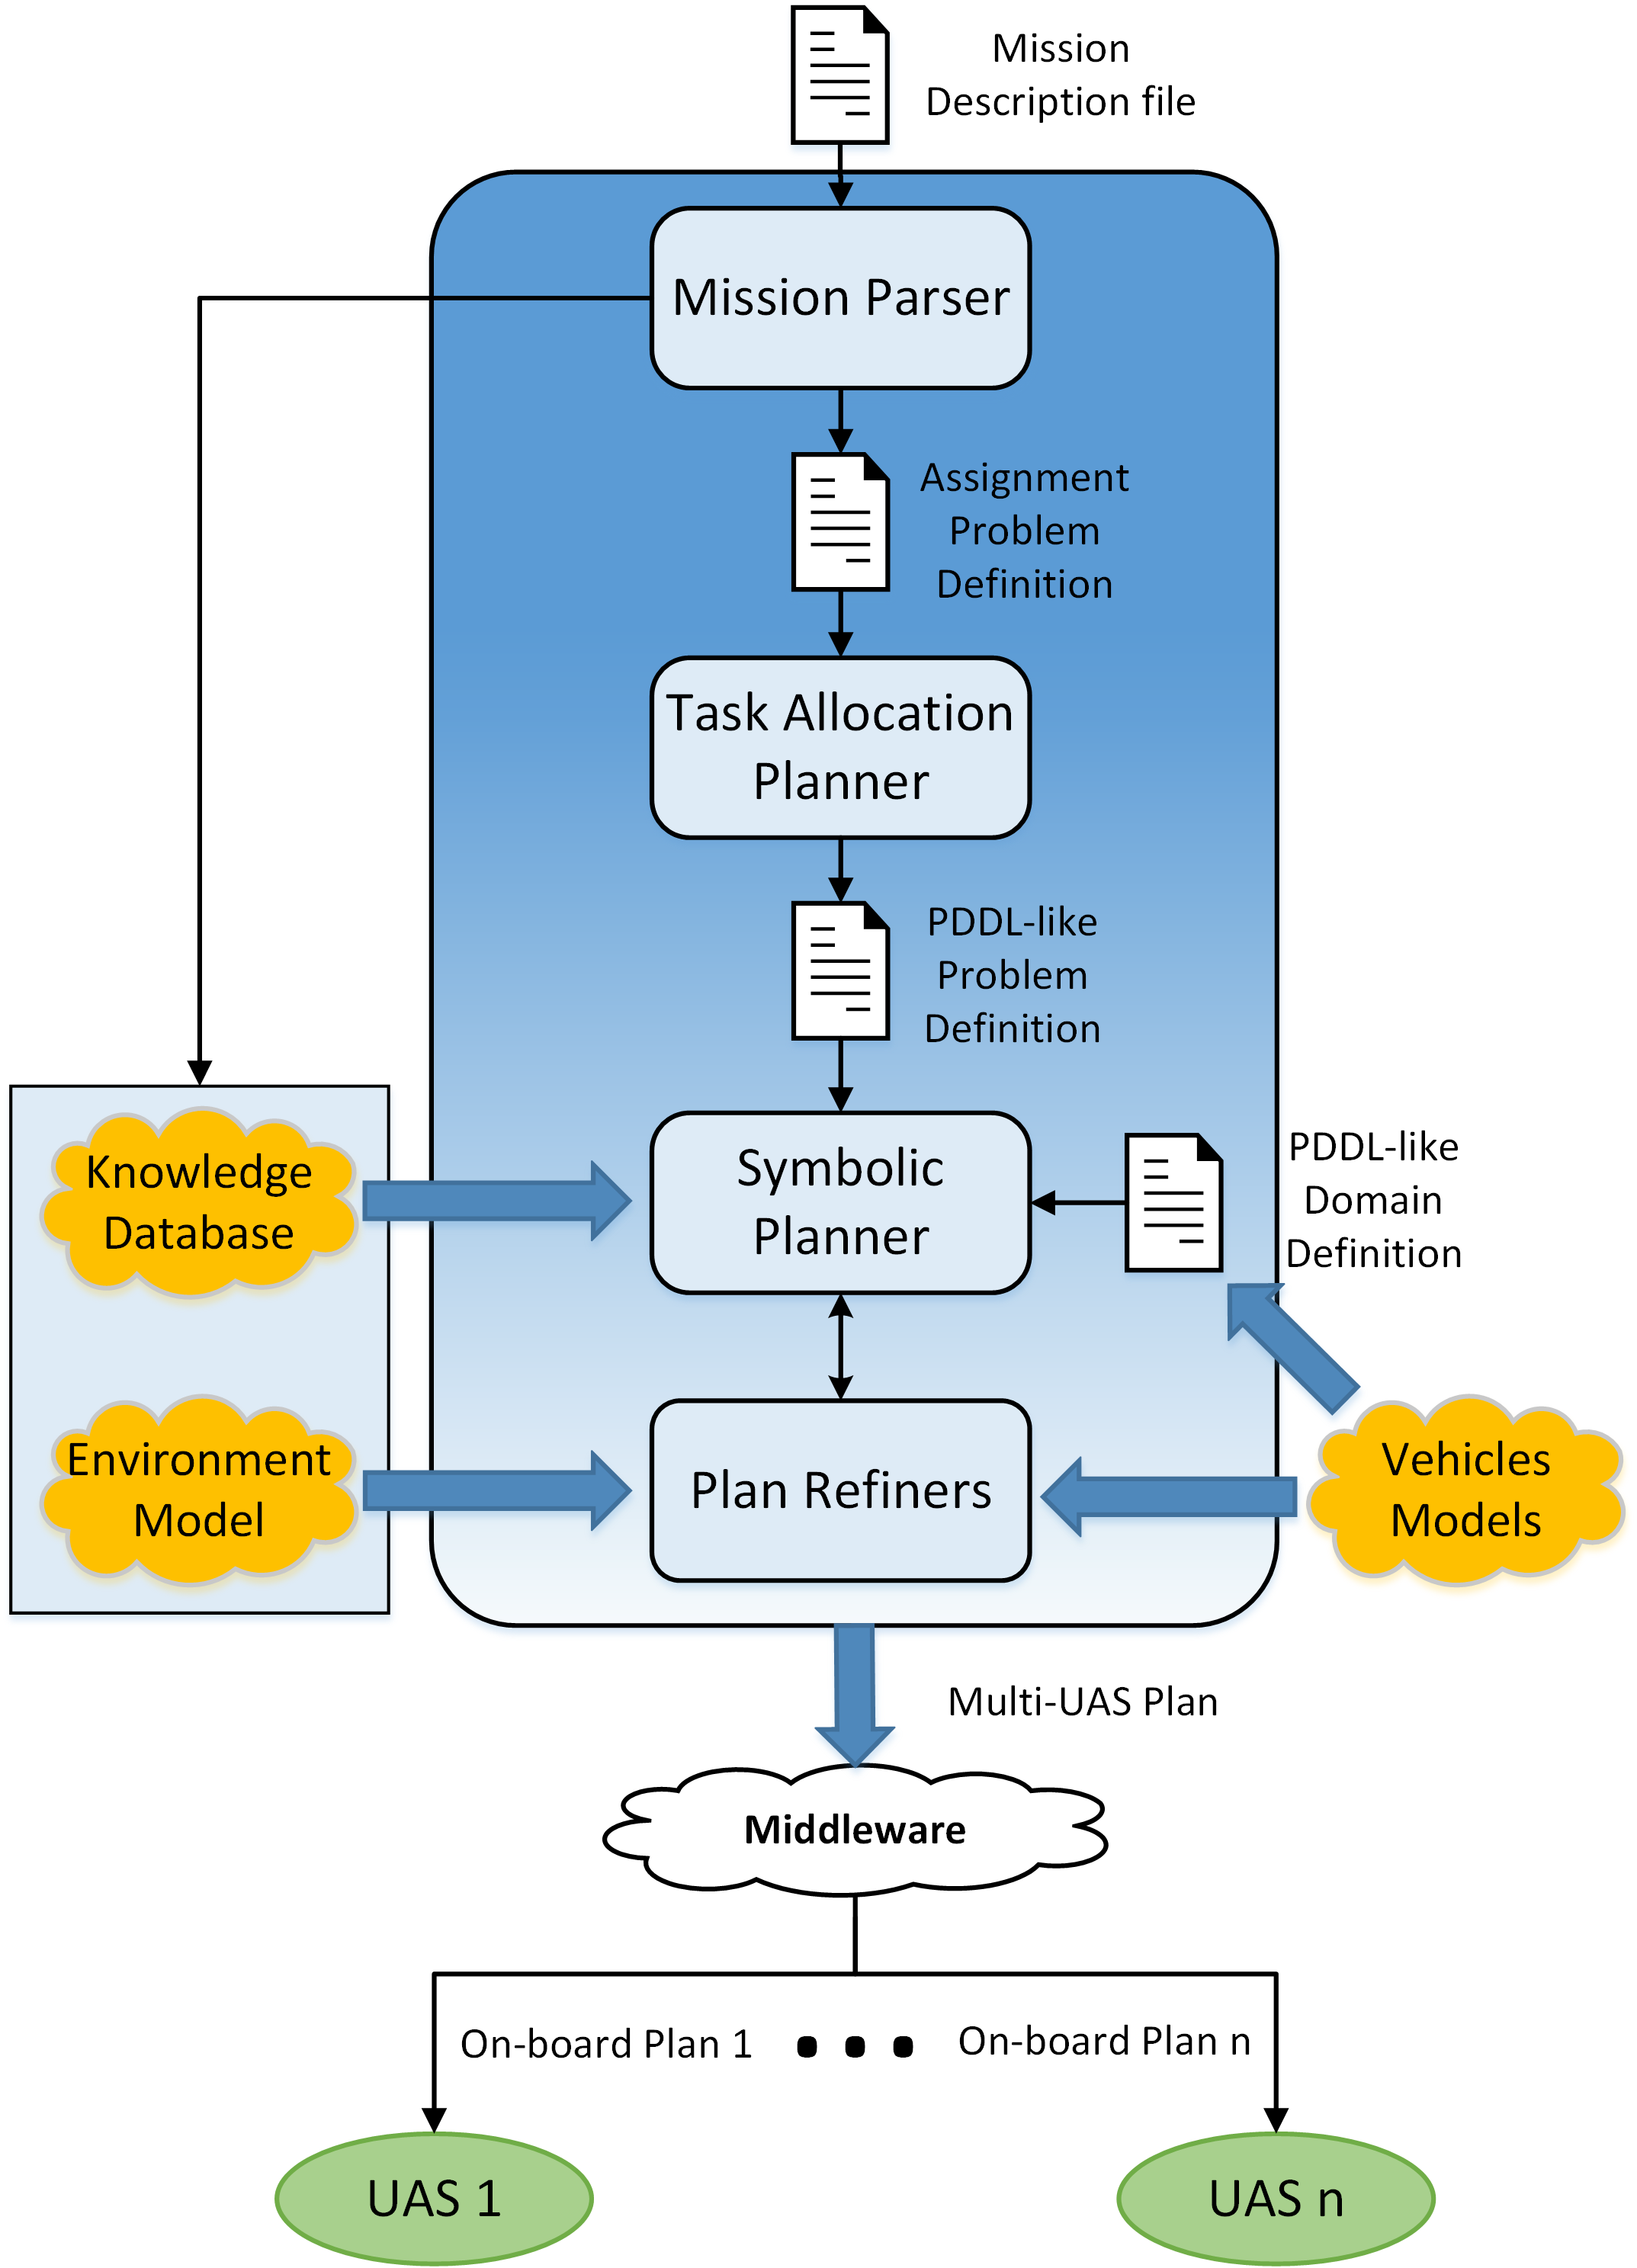
\includegraphics[width=1.0\columnwidth]{global_arch.png}
    \caption[Software architecture of the planning system.]{Software architecture of the planning system.}
    \label{fig:global_arch}
\end{figure}

Both the TAP and the SP receive as input a file defining the problems they have to solve, and hence two additional modules should be present in the architecture. These modules are parsers that adapt the format of the information in order to be understable by each of the planners. Finally, the output of the architecture is a plan that contains the set of primitives for each of the UAS involved in the mission, called on-board plans. That plan can be examined by the user and its execution can be monitored on a Ground Control Station.

The main components presented in this section are described with more details in the following subsections.

\section{Mission Parser}
    \label{sec:mdlp}

The input of this module is a mission file, i.e a XML text file that contains the C-BML description of the mission, as well as all the related data. This module consists on a C-BML language parser implemented in C++ that can parse single or multiple files and can determine if the content of the files are compliant with the C-BML standard. The library used for the parser implementation was CodeSynthesis XSD. This library is released under GNU General Public License (GPL) version 2 and is an open-source, cross-platform W3C XML Schema to C++ data binding compiler. Starting from the XML Schema definition of a XML language, it generates C++ classes that contain the necessary data types and functions to access all the data stored in the XML files that will be parsed, without having to work directly with the DOM (Document Object Model). From the set of all XSD Schema files that compose the C-BML standard specification, different C++ classes have been generated automatically and by using these classes the parser has been implemented. 

If the files are not valid C-BML orders, message errors are displayed and the process terminates. If the files are valid C-BML orders, then a new file is generated containing an assignment problem in a format that the task allocation planner can understand. An example of a C-BML order can be seen in  Listing~\ref{cbml_example}, whereas the format generated by the mission parser will be explained in the next subsection.

\lstinputlisting[label=cbml_example,caption=Simplified C-BML order representing a surveillance task for a fleet of UAS (activity code SURVLE).]{cbml_example.xml}

\section{Task Allocation Planner (TAP)}
    \label{sec:tap}

This component is responsible of generating an initial assignment for the tasks that compose the mission to the available UAS. In order to generate this initial assignment, the TAP needs the assignment problem expressed in a suitable format generated by the mission parser. This section contains the problem definition and the details about how this planner solves it.

\subsection{Problem Description}
    \label{sec:pdesc}
    
    Let us consider a mission $\mathcal{M}$ composed by a set of unordered tasks $\mathcal{T}$ where each of them have to be performed on given locations by a team of UAS starting the mission on their home locations. Let us define $\mathcal{L}$ as the set of locations where the tasks have to be done, $\mathcal{L'}$ as the home locations of the UAS and $n$ as the number of UAS available for the mission. The objective is to execute all the tasks on their locations minimizing the travel time of the vehicles. In addition to the travel time, the execution time cost of the tasks has also to be considered.
    
    The implicit combinatorial problem can be expressed by the edges of a graph $G(V,E)$ considering the following notation:
    
    \begin{itemize}
    	\item $\mathcal{T} = \{t_1, t_2, ..., t_m\}$ is the task set.
    	\item $n$ is the number of UAS.
    	\item $\mathcal{L} = \{l_1, l_2, ..., l_m\}$ is the task locations set.    	
    	\item $\mathcal{L'} = \{l'_1, l'_2, ..., l'_n\}$ is the UAS home locations set.
  		\item $V=\{\mathcal{L}\cup\mathcal{L'}\}=\{v_1, v_2, ..., v_{n+m}\}$ is the vertex set of the graph.
		\item $C$ is a matrix of non-negative costs or travel times $c_{ij}$ between vertex $v_i$ and $v_j$, where $c_{ij}=c_{ji}$.
		\item $E=\{(v_i,v_j) | v_i,v_j \in V; i<j\}$ is the edge set.
		\item $d = \{d_1, d_2, ..., d_m\}$ is a vector of execution time costs for the tasks.
		\item $w = \{w_1, w_2, ..., w_n\}$ is a vector of the maximum flight times for the UAS.
		\item $R_i$ is the route for the $i$-th UAS.
	\end{itemize}
	
	The problem consists of determining a set $\mathcal{R}$ of UAS routes with minimal cost, each starting at the home locations of the vehicles, such that every vertex in $\mathcal{L}$ is visited at least by one vehicle, without exceeding the maximum flight time of each of the vehicles involved. The possibility of visiting the same location with multiple UAS is given by the fact that some tasks may be done cooperatively by distinct UAS. The problem described is similar to the well-known Vehicle Routing Problem (VRP).
	
	The cost of a given route ${R_{i} = \{v_0, v_1, ..., v_s}\}$ is given by 

 \begin{equation}
 	{C(R_{i}) = \sum_{i=0}^{s-1} c_{i,i+1} + \sum_{i=1}^{s} d_{i}} \, ,
 	\label{eq:route_cost}
 \end{equation}	

\noindent where ${v_i \in V}$ and ${v_0 \in \mathcal{L'}}$.

	A route ${R_{i}}$ is feasible if the given UAS visit each task location exactly once and the sum of the task execution time costs does not exceed the maximum flight time for the UAS, i.e. $\sum_{i=1}^{s} d_{i} \leq w_i$. The goal of the planner is to minimize the total travel time $\sum_{i=1}^{m} C(R_{i})$ of the feasible routes executing of the tasks of the mission.
	
\subsection{Problem Solver}
    \label{sec:opt}
    
The planner chosen to solve the assignment problem presented in the previous subsection was OptaPlanner~\cite{optaplanner}, an open source, multi-platform planning engine written in Java and released under Apache Software License. OptaPlanner is aimed to solve planning problems with resource usage optimization. It is capable of generating near-optimal plans by applying optimization heuristics and meta-heuristics combined with score calculation. One of his main advantages is that the solver's algorithm is highly configurable. In OptaPlanner it is possible to use different heuristics and meta-heuristics algorithms applied in sequence, so that the user can select the most suitable for the problem in question. These algorithms tell OptaPlanner how the planning entities should be planned while the planning process is running. The optimization is done in base of a score calculation that is computed after all the planning entities have been assigned. This score determines the suitability of the last computed solution: if after searching for a new solution, the new score is higher than the score calculated in the previous solution, then the last solution is discarded and the process continues trying to generate a solution with a lower score.

As it was mentioned above, the OptaPlanner solver can use multiple optimization algorithms in sequence. Each of the optimization algorithms used is called a solver phase. During the execution of the solver there is never more than one solver phase executing at the same time, so a solver phase only starts when the previous phase has finished. There are three types of solver phases that can be used in the OptaPlanner solver: Construction Heuristics (CH), Metaheuristics (MH) and Exhaustive Search (ES). 

The CH solver phase builds an initial solution in finite time. The solution computed is not always feasible, but it tries to find it fast so that the following solver phases can finish the searching of a feasible one by starting from that initial solution. There are different algorithms that can be used as CH. One common characteristic of them is that when a CH assigns a planning variable, that assignment remains unchanged until the end of the algorithm. This is the main reason that makes the CH algorithms find solutions that may be unfeasible: no re-planning is done at this phase.

The MH phase is based on different types of local search algorithms. Local search starts from the initial solution computed by the CH phase and evolves that into a mostly better and better solution. At each solution, it evaluates a number of moves between the planning entities of the solution and applies the most suitable to step to the next solution, whose score has to be equal or better (lower) than the previous. One important thing to be taken into account is that the local search does not use a search tree, but a search path. When finding a new solution all possible moves are tried but unless it is the chosen move, it does not investigate further the rest of possible solutions. That makes the local search very scalable, but as a disadvantage it may not find never the optimal solution.

The last ES solver phase does not depend on previous phases and it is applied alone. Brute force or the branch and bound algorithms are available. These methods can find the optimal solution for a problem, but are poorly scalable.

The solver should minimize the travel time (or the distance travelled) by each of the vehicles, not exceeding the maximum flight time of the UAS executing the assigned tasks. That problem had to be defined using the OptaPlanner format. One of the main characteristics of OptaPlanner is that the problems are defined in XML files by using a very intuitive XML notation. These input files have a format that is dependent on the name of the Java classes and attributes that conform the domain designed for the problem. This is due to one internal tool that OptaPlanner uses to parse automatically the problem definition files, having only to check that the names of the XML nodes in the input problem file are equals to the names of the Java classes and attributes that conform the domain of the specific problem to be solved. By this way, all the nodes of the XML file are de-serialized and the corresponding Java objects are created in memory. A simplified example of the input problem file format can be seen in Listing~\ref{tap_example}. The file contains all the locations, starting points, UAS and tasks that should be accomplished. It is important to note that although each task is of a specific type, they are considered to be generic by the TAP because at this level of abstraction, only the estimated execution cost for the tasks is considered.

\lstinputlisting[label=tap_example,caption=Simplified problem file for the Task Allocation Planner. Each node has a XML attribute called 'id' whose value can be used to reference the node from a different node by using the 'reference' attribute. The 'flightTime' and 'cost' node values are expressed in seconds.]{tap_example.xml}

It should be mentioned that one task may be executed by a single UAS or by multiple UAS cooperatively (not necessarily in parallel). The idea is to exploit the capabilities of a team with multiple UAS in the assignment. In order to do so, certain types of tasks are automatically discretized, i.e. the total cost of the task is divided and the workload can be shared in a more balanced way among the UAS. In this manner, if a location associated to a task is visited for instance four times by one UAS and six times by another, it means that the first UAS will take 40\% of the total cost of the task and the other will take the remaining 60\%. If the type of the task is area 3D mappping or surveillance, these percentages will correspond to partitioning the given polygonal area into two subareas with the 40\% and the 60\% of the total size.

After solving the problem, an XML output file that contains the solution is generated in a format that will be discussed in the following subsection. 

\subsection{Allocation Solution Parser}
    \label{sec:sop}

For each XML node that represent the UAS which are present in the input problem and that have at least one assigned task in the computed solution, an 'assignment chain' is created, consisting on one inner XML node with the tag 'nextTask' which contains the next task that the given UAS should execute. That special node can have inside another 'nextTask' node specifying the following task to do after the previous, etc. Thus, this chain contains the ordered locations that the UAS should follow to execute the corresponding tasks. An example of the output file can be seen in Listing~\ref{tap_solution_example} that shows an assignment calculated for a given UAS.

\lstinputlisting[label=tap_solution_example,caption={Part of a task allocation planner solution. Three different tasks appear in the assignment chain of a given UAS. The UAS has one task repeated two times because the location with reference 5 appears in two of its 'nextTask' nodes. Then if this location appears a total of ten times in all the 'nextTask' nodes present in the whole file, this UAS will have a 20\% of the workload for the task.}]{tap_solution_example.xml}

The allocation solution parser has been implemented in Java and generates an output in a format similar to a Planning Domain Definition Language (PDDL) description that contains the initial assignment and can be processed by the symbolic planner described in the next section.

\section{Symbolic Planner (SP)}
    \label{sec:sp} 

This component is the responsible of decomposing the mission tasks into primitives that can be directly executed by the UAS. The symbolic planner has been implemented by using the JShop2 planner~\cite{Nau03shop2}. JShop2 is a Java implementation of the Shop2 planning system. It is a domain-independent Hierarchical Task Network (HTN) planner. As an HTN planner, JShop2 starts its planning process from a problem file which contains the initial state of the world. This file defines all the entities that are present in the problem and their initial state, as well as the tasks that should be accomplished. The objective of JShop2 is the decomposition of these tasks into decreasingly smaller subtasks, until obtaining primitive tasks which are the actions at the lowest level that compose a final plan. JShop2 needs to know how this decomposition has to be done, so an additional file should be given containing the domain of the problem. In this domain the structures that represent the high level tasks (called methods) are defined, as well as the structures that represent the primitives (called operators). The methods contain the list of subtasks on which they can be decomposed, either another methods or operators. Thus for solving the symbolic planning problem these two files, the problem file and the domain file, should be available in a format that is very similar to PDDL, which is generated by the allocation solution parser explained before.

Some of the JShop2 entities present in the problem file are those which represent the locations of interest, the existing UAS and their available batteries. Each battery pertains to a UAS and its numerical value will be decreased each time the UAS execute an action, so every vehicle could do only a finite number of tasks. In addition to these entities, some predicates have been defined for the UAS. These predicates conform the initial state of the vehicles, and its existence may change during plan solving. Each UAS can have three different predicates associated:

\begin{itemize}
  \item At: means that the related UAS is on a certain location, expressed in the predicate.
  \item Landed: means that the related UAS is currently landed.
  \item Idle: means that the related UAS has no initial tasks assigned.
\end{itemize}

From the previous predicates, the two that are present in every step of the planning process are the 'At' predicate and the 'Idle' predicate. All the UAS should be on a specific location at any time, so they always have a related location although this location will change as the vehicle moves. The 'Idle' predicate expresses when a UAS does not have any assigned tasks at the beginning and this information is used by the symbolic planner in case a reassigment is required as it will be explained later. due to any problem detected at this level with a task previously allocated by the TAP.

As commented before, the format of the problem and domain files is very similar to a PDDL definition. However, one of the lacks of JShop2 is that it does not support durative and concurrent actions that are present in PDDL Level 3. However the JShop2 format is expressive enough to represent these type of actions because in the preconditions of the methods and operators of the domain some calculations can be done. There are different techniques to accomplish that but the one used in this work is the explained in~\cite{Nau03shop2}, which is called Multi-Timeline Preprocessing (MTP). By using this technique it was possible to mark each operator with a start and duration stamp. This required to insert in the JShop2 problem definition the read/write times of the predicates whose values could be modified after the execution of a method. The problem file also contains the particular high-level tasks that the system can execute. Each task has associated the location on which the task should be done, the initial UAS assigned and a numeric value representing the workload over the entire task given as a percentage. For a given task, the assigned UAS could be changed by the SP if a re-planning is needed but the rest of parameters will remain unchanged.

The domain file contains the different JShop2 methods that represent the tasks present in the problem file, as well as the other methods and operators on which they can be decomposed. Due to the MTP technique applied, all the operators have a start and a duration stamp, so the final plan is composed by a set of possibly concurrent primitives where the start and end of each primitive is well defined in time.  Listing~\ref{jshop2_map_generation} shows the 'mapGeneration' method as an example. This method appears as a task to be done in the problem file, but its definition is formalized in the domain file.

If at this planning level, any problem with a task previously allocated by the TAP is detected, the task can be reallocated by the symbolic planner. In order to implement this capability, the methods that represent the tasks receive as input parameter the UAS that should execute the task with preference. Inside the preconditions of the method, a list containing all the possible candidates to do the task is created. That list contains in the first position the UAS which has preference to do the task and which was passed as a parameter, followed by the set of UAS tagged with the 'Idle' predicate. Then the sub-tasks of the method are tried by JShop2 choosing the different UAS that compose the list in the given order. That makes that, if the UAS with preference fail in any of the sub-tasks of the method, then the rest of UAS in the list tagged as 'Idle' will be checked. This is the way the reassignment has been implemented in our domain. An example is illustrated also in Listing~\ref{jshop2_map_generation}.

\lstinputlisting[label=jshop2_map_generation,caption=Implementation of the JShop2 'mapGeneration' method corresponding to 3D map generation task.]{jshop2_map_generation.txt}

One important feature of the JShop2 implementation is the possibility to call external Java code from inside the preconditions of the method definitions. This is useful when the planner needs access to the environment model. When decomposing a task to obtain its primitives, the planner needs to know information about the environment like the extension of the area where the task has to be done or the obstacles around. This information is required to estimate the cost of executing the subtasks that compose a task or to check the feasibility of moving a vehicle between locations. The external Java calls reduce the complexity of the JShop2 domain by freeing the planner of the need to have all the geometric information encoded inside the problem file. These geometric reasoning operations are delegated to the plan refining tools component described in the next section by using external Java calls within the JShop2 domain. These calls allow for instance to receive in the preconditions the detailed travelling cost of a task taking into account the obstacles present in the environment.

\section{Plan Refining Tools}
\label{sec:prt}

The Plan Refining Tools (PRT) component contains different software tools with geometric reasoning functionalities. The symbolic planner in Fig.~\ref{fig:global_arch} interacts with this component to compute geometric data for plan refinement and execution. 

One of the tools embedded in this component is a path planner required by the symbolic planner to check whether a certain UAS can travel from one location to another avoiding obstacles. The path planner generates a path free of obstacles for the execution and estimates the cost of the motion for the symbolic planner. The path planner used in this paper is based on the path planning module present in V-REP~\cite{vrep_iros13}. The Environment Model of this architecture (see Fig.~\ref{fig:global_arch}) has been created as a V-REP scene that contains all the UAS, locations and objects of interest in the mission. A V-REP client application has been developed by using the V-REP C++ remote API to connect the symbolic planner with the path planner. That client application communicates with a V-REP server developed by using the LUA language in a embedded script. That client is invoked from the JShop2 planning process with external Java calls when the symbolic planner needs to know if a certain vehicle can travel from one location to another. The query is done by the client and processed by the server, which in turns makes a call to the V-REP path planner module to check if there is any path free of collisions between the locations. The length of the path is returned (or a negative number if there is no path free of collisions) and the path itself is stored for later use in the execution.

Other tools embedded in this component are more specific for some particular tasks. For example for cooperative area surveillance or 3D mapping tasks, the area of interest can be divided among different vehicles according to their capabilities. Then each sub-area should be covered by a vehicle following a given pattern. In order to tackle with these geometric computations, two specific tools based on the work presented in~\cite{maza_dars07} have been developed:
\begin{itemize}
\item Area partition computation: given an area with no-fly zones inside, this tool divides the area in different sub-areas. The size of each sub-area depends on the percentages computed by the task allocation planner to perform the area related task in a cooperative manner.
\item Coverage pattern generation: this tool generates a zigzag pattern for a vehicle equipped with sensors on-board covering a given area.
\end{itemize}
 
Finally it should be mentioned that the set of tools implemented can be adapted and/or extended depending on the particular capabilities of the vehicles. 

\section{Architecture Application Example}
\label{sec:results}

In this section a representative mission will be used to illustrate the operation of the architecture in a multi-UAS context. In the mission presented, a fleet composed of five unmanned aerial vehicles is available, where four of the vehicles are simulated and the leftover is a real quadrotor. The environment contains twelve locations of interest (see Fig.~\ref{fig:locations}) around the Cartuja Campus (University of Seville - Spain) where five of them are home locations of the UAS. The mission is composed by three tasks of type surveillance and four 3D map generation tasks which have to be performed in disparate locations. 

At \verb+http://grvc.us.es/jint2015grvc+ the reader can find the C-BML files, the assignment problem for the TAP, the planning problem for the SP, the intermediate files and the planning results generated by the system, as well as a video showing the execution of the plan computed for the real quadrotor.

\begin{figure}
    \centering
    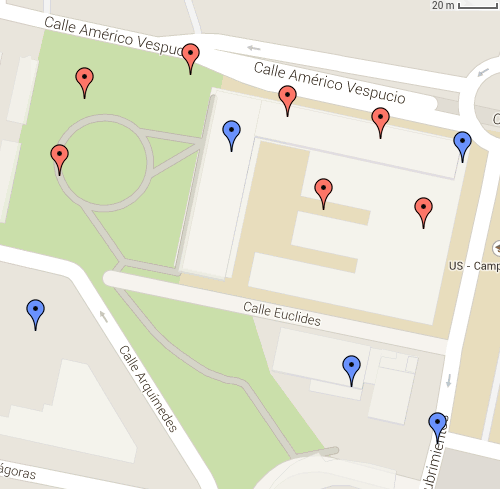
\includegraphics[width=1.0\columnwidth]{mission.png}
    \caption[Locations involved in the mission.]{Locations involved in the mission. The locations with the blue marker are the home locations of the UAS whereas the other locations are related to the tasks to be performed.}
    \label{fig:locations}
\end{figure}
 
The entry point to the system is the description of the mission in C-BML provided by the user. For example, Listing~\ref{map_task} shows the C-BML expression that defines a 3D map generation task. 

\lstinputlisting[label=map_task,caption={C-BML expression for a 3D map generation task composed by the required 'What', 'Where', 'When' and 'Who' C-BML structures, with the optional 'Why' structure omitted for the sake of simplicity. The 'MAP' activity code  defines in C-BML an action 'to create a graphic representation, usually on a plane surface and at an established scale, of natural or artificial features on the surface of a part or the whole of the earth or other planetary body'.}]{map_task.xml}

The location where the task starts, a single geographic point with specific GPS coordinates, is defined in the 'Where' structure. The 'When' structure specifies to start the task as soon as possible (ASAP). Additionally, the maximum duration of the task is defined with the ENDSNL (ends no later) category code. Finally, the 'Who' structure is composed by the Tasker which commands the mission, the Command and Control unit, and by the Taskee who executes the mission, our fleet of UAS. It is important to notice that the task is commanded to the whole fleet of UAS and not to a specific vehicle. The task allocation planner automatically computes the allo

The mission parser reads the C-BML description and generates an assignment problem for the task allocation planner with the definition of the following entities: 

\begin{itemize}
  \item Locations: the different points of the environment where the tasks have to be executed.
  \item Starting points: the home locations of the UAS.
  \item UAS: the available vehicles to perform the mission with their associated home locations and the maximum estimated flight time according to their battery levels.
  \item Tasks: the tasks of the mission with their types, locations and estimated costs (durations).
\end{itemize}

In the assigment problem, the user can add safety constraints such as the maximum percentage of battery that can be devoted to the execution of the tasks. The restriction aims to reserve a given percentage of the battery for unexpected deviations from the nominal execution of the tasks. In the results presented in this section, the user imposed to consume a maximum of 50\% of the total battery reserve. Then for an estimated battery life of 20 minutes, the maximum flight time for each UAS would be 600 seconds.

As it has been previously commented in Section~\ref{sec:opt}, in order to exploit the capabilities of a team with multiple UAS in the assignment problems certain types of tasks can be discretized to be shared among different UAS. For instance in this example the second task of the mission has a cost of 341 seconds and it has been automatically discretized into six parts, each one with a maximum cost of 60 seconds (see Listing~\ref{task_discretization}). 

The task allocation planner solves the assigment problem generated by the mission parser and computes the solution shown in Fig.~\ref{fig:solution_optaplanner}.  It can be seen that the tasks are assigned to their closer vehicles, and the task with highest cost is shared between two UAS. The solver was configured to apply two phases: a Construction Heuristic and a Metaheuristic. The Construction Heuristic chosen was the so called First Fit Decreasing, which assigns the more difficult planning entities first (those tasks with a higher cost in our case), so it sorts the planning entities on decreasing difficulty. The Metaheuristic chosen was the Late Acceptance, a variant of the Hill Climbing local search. Late Acceptance does, for the assignment initially computed by the Construction Heuristic, some moves between the planning entities, one per iteration, and accepts any move that leads to a score that is better than the best score of a number of moves ago. This allows to do one move that initially leads to a worse score than the previous to improve the score calculated some moves ago. 

\lstinputlisting[label=task_discretization,caption=Task discretization generated by the mission parser for the second task of the mission.]{task_discretization.xml}

\begin{figure}
    \centering
    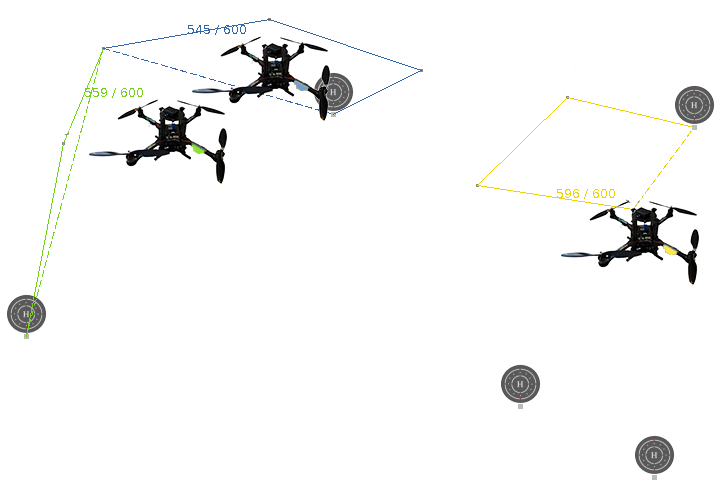
\includegraphics[width=1.0\columnwidth]{solucion.png}
    \caption[Solution computed by task allocation planner.]{Solution computed by the task allocation planner. Only three UAS are used in the solution and the location visited two times represents the task with highest cost that has been assigned to two different UAS to be completed cooperatively.}
    \label{fig:solution_optaplanner}
\end{figure}

After the initial assignment problem has been solved, the solution parser generates a planning problem in a format suitable for the symbolic planner based on JShop2. This JShop2 planning problem contains the high level tasks that should be decomposed into primitives, as well as the initial states of all the entities involved. Listing~\ref{jshop2_prob} shows the planning problem generated for our mission containing the sub-areas computed by the area partition tool with their associated covering costs (see Section~\ref{sec:prt}). 

\lstinputlisting[label=jshop2_prob,caption=Input problem for the symbolic planner.]{jshop2_prob.txt}

The plan computed by the symbolic planner contains all the primitives for each of the UAS involved in the mission execution and it has been represented with a Gantt chart in Fig.~\ref{fig:sp_gantt_solution}. The symbolic planner makes queries to the V-REP path planner to check if there is a path avoiding obstacles between the locations that should be traversed by the different UAS. A non-fly volume defined by the user in the environment model prevents the execution of a task assigned to one of the UAS. This condition is detected by the symbolic planner, which modifies the initial assignment generated by the TAP and reallocates it to one of the UAS that was initially idle. Thus four UAS are finally involved in the execution of the mission.

\begin{figure*}
    \centering
    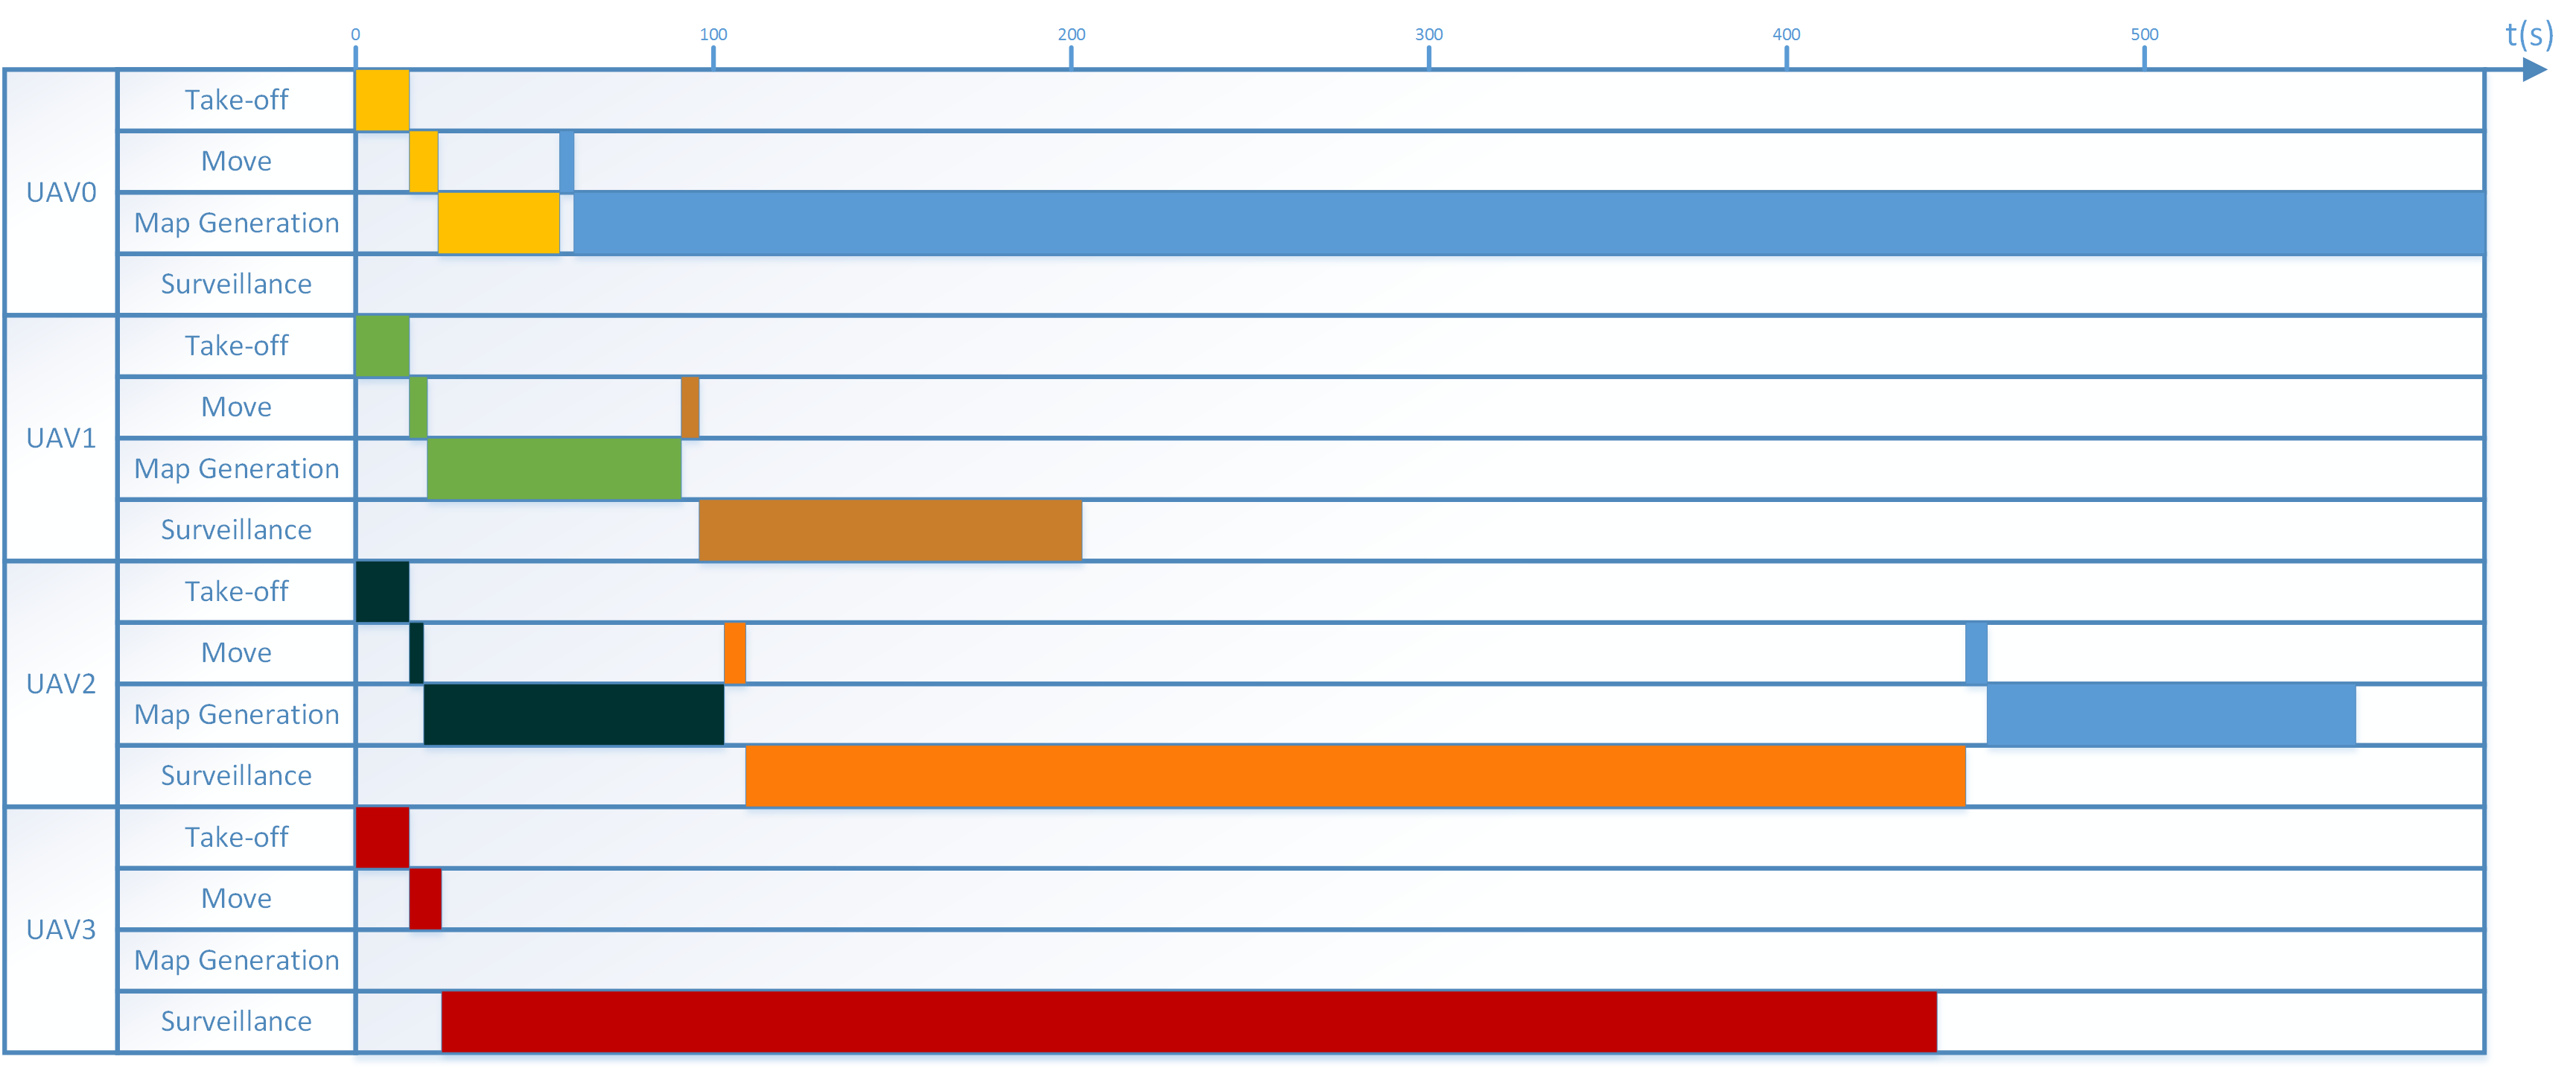
\includegraphics[width=0.99\textwidth]{sp_gantt_solution.png}
    \caption[Gantt chart of the final plans computed by the symbolic planner.]{Gantt chart of the final plans computed by the symbolic planner. Each rectangle represents a primitive, while each color represents a task. Then, primitives of the same task have the same color. The task in light blue color appears in the timeline of two UAS because they share its execution. It should be noticed that a cooperative task does not imply that the task have to be executed concurrently in time by the different UAS. Each assigned UAS start its part of the task when it fits better in its own plan.}
    \label{fig:sp_gantt_solution}
\end{figure*}

A video with the execution of the 3D map generation task that was assigned by the system to the real UAS (UAV 0) can be dowloaded from the previously mentioned web site. Figure~\ref{fig:exp:exp8_screen} shows several screenshots of the Ground Control Station during the execution with some overlays providing additional information.

\begin{figure}[htbp!]
    \centering
	\subfigure[Polygonal area and zigzag coverage path computed for the 3D map generation task.]{
	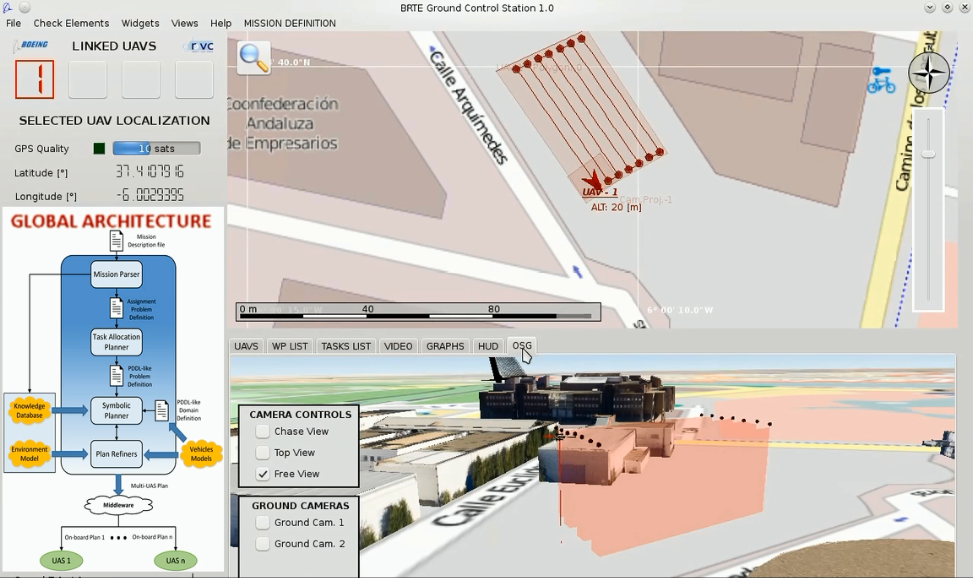
\includegraphics[width=0.99\columnwidth]{video1.png}
	\label{fig:exp:exp8_screen_1} } \subfigure[Orthophoto computed after the execution of the task.]{
	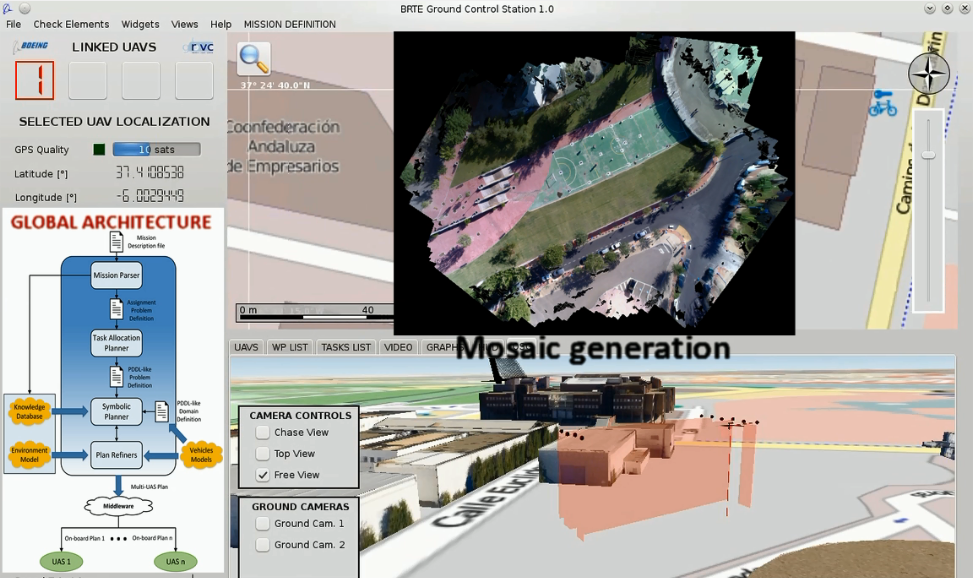
\includegraphics[width=0.99\columnwidth]{video2.png}
	\label{fig:exp:exp8_screen_2} } \subfigure[Coloured 3D point cloud generated after the execution of the task.]{
	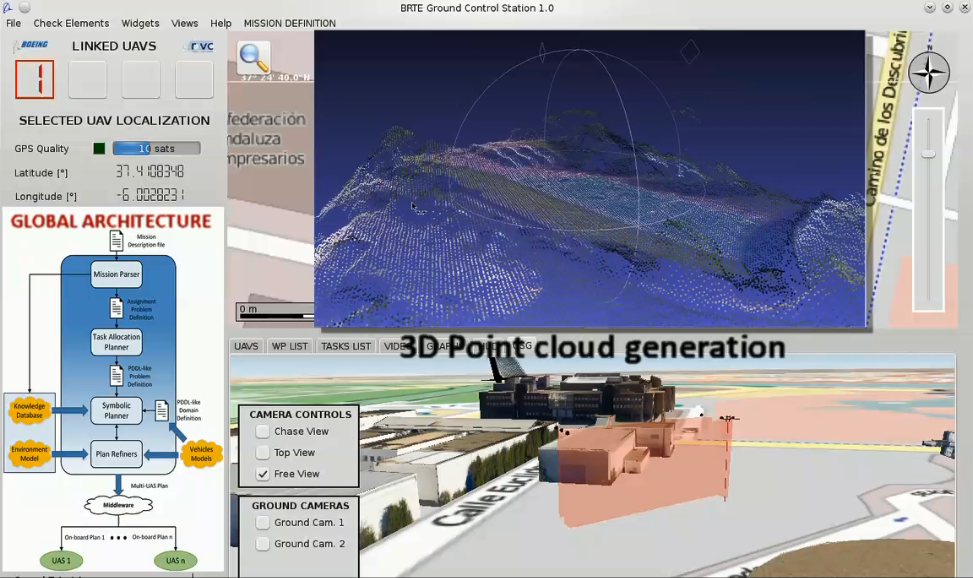
\includegraphics[width=0.99\columnwidth]{video3.png}
	\label{fig:exp:exp8_screen_3} } \caption[Screenshots of the Ground Control Station during the execution of the 3D map generation task allocated to the real quadrotor (UAV 0 in Fig.~\ref{fig:sp_gantt_solution}).]{Screenshots of the Ground Control Station presented in~\cite{perez_jint13} during the execution of the 3D map generation task allocated to the real quadrotor (UAV 0 in Fig.~\ref{fig:sp_gantt_solution}). The different elements in the interface are: the telemetry of the quadrotor (left), the 2D map view (right) and the 3D map view (bottom).}
    \label{fig:exp:exp8_screen}
\end{figure}

\section{Conclusions and Future Work}
	\label{sec:conclusions}

A planning approach for a platform composed of multiple unmanned aerial systems has been presented in this paper. The research activities has been focused on the interoperability, task allocation 
and task planning problems within the system. The main contribution of the paper is the capability of the system to automatically generate low level plans for each of the vehicles from a mission described in C-BML. The architecture integrates symbolic, geometric and task allocation planners.

The current system includes offline replanning capabilities. For instance, when the symbolic and geometric planners detect that a task can not be executed by a given vehicle, a new assigment is checked. However, these capabilities should be extended in order to allow online replanning in case of problems during the execution of the missions. On the other hand, the architecture should be tested under a wide spectrum of missions and tasks. The goal is to check how general are the different components and which is the level of customization required.

Finally the approach has been tested in missions involving multiple surveillance and 3D map generation tasks with a team of simulated and real UAS. In future work the goal is to increase the number of real UAS in order to find more realistic adn complex contexts to test the architecture developed. 


%-----------------------------------------------------------------------------
% BIBLIOGRAPHY
%-----------------------------------------------------------------------------
% BibTeX users please use one of
%\bibliographystyle{spbasic}      % basic style, author-year citations
%\bibliographystyle{spmpsci}      % mathematics and physical sciences
%\bibliographystyle{spphys}       % APS-like style for physics
%\bibliography{}   % name your BibTeX data base
\bibliographystyle{spmpsci}
\bibliography{IEEEabrv,bibliography}

\end{document}